\documentclass[12pt,a4paper]{scrartcl}

\usepackage[english]{babel}
\usepackage[T1]{fontenc}
\usepackage{graphicx, subfig}
\usepackage[document]{ragged2e}
\usepackage{lmodern}
\usepackage{color}
\usepackage{amsmath}
\usepackage{graphicx}
\usepackage{amsmath}
\usepackage{amsfonts}
\usepackage{amssymb}

% Für Verwendugn von Utnerstrichen ohne Escaping
\usepackage{underscore}

% Für Referenzen mit eigenem Text
\usepackage{hyperref}

% Für Codeblöcke
\usepackage{listings}

% Für Verwendung von Farben
\usepackage[usenames,dvipsnames,svgnames,table]{xcolor}

% Für Verktor-Pfeile
\usepackage{esvect}

% Für Größe der Seitenränder
\usepackage[margin=1in,footskip=0.5in]{geometry}

% Für Tabellen über Seiten hinweg
\usepackage{longtable}

% Für Header and Footer
\usepackage[automark]{scrpage2}

% Für Bildunterschriften
\usepackage[aboveskip=2pt]{caption}

% Formatierung für Hyperref-Referenzen
\hypersetup{
	colorlinks,
	linkcolor={blue!50!black},
	citecolor={blue!50!black},
	urlcolor={blue!80!black}
}

% Generelle Formatierung für Code-Blöcke
\lstset{ %
	columns=fullflexible,
	keepspaces=true,
	frame=single,
	breaklines=true,
	breakautoindent=true,
	gobble=0,
	tabsize=2,
	belowskip=0pt
}

% Formatierung für Pseudo-Code
\lstdefinelanguage{PSEUDO} 
{ 
	xleftmargin=0pt, 
	xrightmargin=0pt,
	basicstyle=\small\ttfamily\color{Black},
	morekeywords={for, each, if, else},	
	keywordstyle = {\color{Orange}},
	sensitive=false,
	morecomment=[l]{//},
	morecomment=[s]{/*}{*/},
	morestring=[b]"
}

\newcommand{\mybox}{%
    \collectbox{%
        \setlength{\fboxsep}{1pt}%
        \fbox{\BOXCONTENT}%
    }%
}
\makeatother
\title{Water simulation in OpenGL}
\author{Fabian Niehaus, Tuyet Nguyen}
\date{Juni 22, 2018}

\makeatletter

%% Generelle Kopf- und Fußzeilendefinition
\pagestyle{scrheadings}
%\automark[section]{subsection} 
\clearscrheadfoot
\ihead[]{\@title}
%\ohead[]{\rightmark}
\ifoot[]{\@author}

\begin{document}

\begin{titlepage}
	\centering
	\ \\[2cm]
	{\huge\textbf{\@title}} 
	\\[3cm]
	\large
	\textbf{Field of study:} Media informatics \\
	\textbf{Semester:} 4
	\\[2cm]
	\textbf{Date}: \@date
	\\[2cm]
	\textbf {Authors:}
	\\Fabian Niehaus
	\\Tuyet Nguyen
\end{titlepage}

\newpage
%% Seitezahl auf 0 setzen
\setcounter{page}{0}
\tableofcontents
\newpage
\listoffigures

\newpage
%% Seitennummern einblenden
\ofoot[]{\pagemark}
\normalsize

\section{Abstract}
In this project we will build a C++ application to simulate circular waves on a 3D mesh surface. We will also simulate reflection using the Image Source Method. We will use QT Creator for programming, QT for window management and OpenGL for 3D rendering.

\section{Wave theory}
An obvious way to represent waves is through sine or cosine functions. If one chooses the parameters wavelength, amplitude and wave direction with a certain variance around specified basic values and superimposes a number of these waves, this results in at least one water-like wave train. The following formula results for a sum of sine waves, which are visualized by the Heigth Field H. The water is at rest in the x / z plane of a coordinate system.\\

In this project, we will use a basic cosine wave with variable parameters for amplitude, wavelength and point of origin (POI). A cosine wave with circular expansion can be calculated using the formula

$$P(x,z,t) = a * \cos(k * {\Delta}O + \Phi) $$
\captionof{figure}{MATH!}
\ \\
where \textit{a} describes the wave's amplitude, \textit{k} describes the wave number, ${\Delta}O$ describes the distance to the wave's POI and $\Phi$ describes the phase shift.\\
\ \\
\begin{center}
	\begin{tabular}{ll}
		Wavelength: & $l$ \\
		Time: & $t$ \\
		Wave Number: & $k = \frac{2\pi}{l}$ \\
		Phase Shift: & $\Phi = -2 * \pi * f * t$ \\
		Frequency: & $f = \frac{c}{l}$ \\
		Phase Velocity: & $c = g * l * 2\pi$ \\
		Gravitational Acceleration: & $g = 9.81 m/s^2$
	\end{tabular}
	\captionof{table}{MORE MATH!}
\end{center}
\ \\
As this project aims for a somewhat realistic behaviour of the wave, the amplitude needs to diminish with increasing distance to the wave's point of origin. In order to accomplish this effect, the distance to POI is factored in a second time:

$$P(x,z,t) = a * \cos(k * {\Delta}O + \Phi) * \frac{1}{{\Delta}O+1} $$
\captionof{figure}{MORE MATH!}
\ \\
As ${\Delta}O$ equals $0$ at the wave's POI and multiplier always need to be less than $1$, 1 is added to ${\Delta}O$ in the multipliers divisor.\\
\ \\
Using this formula, the height for every point of a mesh can be calculated.\\


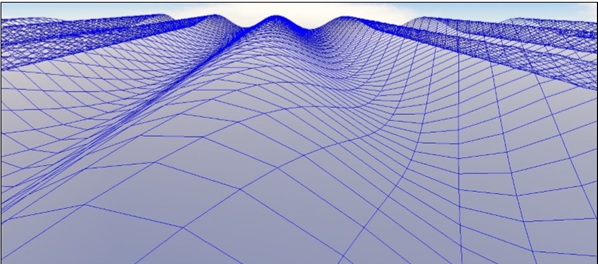
\includegraphics[width=0.7\textwidth]{Images/SinWaves.jpg}
\captionof{figure}{Determining adjacent quads (pseudo code)} 


\section{Realisation}

\subsection{Creating an interface with QT}
First off, we create a new QT widget application. This allows us to use QT Creators design feature to set up our application's interface. A new QOpenGLWidget is placed and will be used as a placeholder for a new custom class inheriting QOpenGLWidgets functionality. This class, called OGLWidget, needs to implement the following methods: initializeGL (for setting up OpenGL), paintGL (for doing the actual rendering) and resizeGL (for handling resizes of the display window). Additionally, the functions stepAnimation SetMaterialColor and InitLightingAndProjection\footnote{Taken from Prof. Dr. Martin Hering-Bertrams OpenGL_Example} are used.

\subsection{Creating the data structure}
The data structure is separated in different classes. \\
The basic class "Waves" contains the contains the information of the waves like sine waves, Height-Field, coordinate, direction vector, phase velocity, the frequency and the wave number.  \\ 
The class "Wavesurface" contains the wavesfunction . 
Logic and data regarding the computation of quad meshes is stored in a seperate class, as are Bezier surfaces and rotational sweep surfaces. \\
In order to allow for easier use of a two dimensional matrix of vertices, a wrapper class containing a two dimensional vector of vertices is introduces. \\


\subsection{Creating the surface mesh}
After creating the required data structure, a method to make a mesh for the waves.\\
Custom data structure\\
2-dimensional vector of QVector3D\\
Dimensions: 50 x 50 -> Best result\\

\subsection{Calculating the wave height}
\begin{lstlisting}[language=PSEUDO]
for each quad
for i = 0 to 3 // since each quad has 4 vertices
a = index of vertex at i
b = index of vertex at (i+1)%4
for each quad that is not the current one
compare all vertices to a and b
if a and b have a match
add index of quad to current quads list of neighbors at index i 
\end{lstlisting}
\captionof{figure}{Determining adjacent quads (pseudo code)} 

\subsection{Rendering as a wireframe}
Depending on the desired way of rendering the object, different draw methods are implemented. These methods are then being called from the paintGL() function.

\subsection{Rendering as an opaque surface}
After drawing the object as a wireframe we want to draw it as a solid cube with lighting. This is being achieved in the method drawQuads() which once again iterates over the list of quads. This time using GL_Quads, the four vertices of a quad are connected and the area inbetween is filled. The normal vector for this is calculated using the cross product of the two diagonals vectors.

\subsection{Reflection}

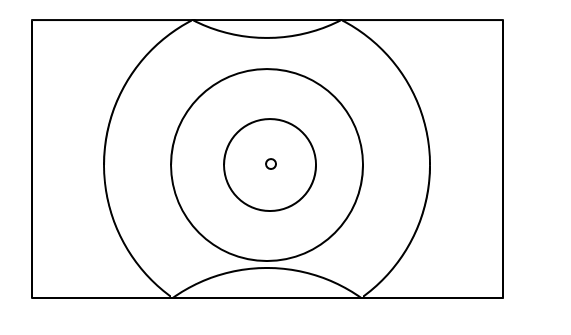
\includegraphics[width=0.7\textwidth]{Images/Reflextion.png}
\captionof{figure}{Determining adjacent quads (pseudo code)} 




\end{document}